%!TEX root = ../../../../report.tex

\subsection{Custom controllers} % (fold)
\label{sub:example_controllers}
From the \textit{Controller manager} in ROS Control, a variety of joint handlers are offered.
Among them, in the created controllers \textit{Impulse controller} and \textit{Two-neuron controller} the position and effort handlers are used individually for each joint.
Thus, these controllers provide a ROS topic (e.g. /rubi/left\_ankle\_position) that the user can employ to move the actuators or read from the sensors.
The joint handlers are created from a unique package called \textit{rubi\_joint\_controllers}.
It is worth mentioning here that the position handlers used for the joints contain a PID whose values have been adjusted experimentally through the simulations for each joint.

Two type of controllers are given that show a different range of options to use with the robot.
Both are gathered in a sole package called \textit{rubi\_controllers}, which gives a more organized and resource-shared environment rather than having a package for each controller.
This also eases the creation of packages for new custom controllers by providing an example package.
In order to start a new piece of code this must be created and then added in the \textit{CMakeLists.txt} from where also some examples are included.
The presented code follows the ROS conventions and the code style is the \textit{Google style} offered by the clang-code-model.
This creates a congruent workspace monitored by a git repository.

\subsubsection{Two-neuron controller} % (fold)
\label{ssub:two_neuron_controller}
This first example controller shows how to:
\begin{enumerate}
    \item Use GoRobots.
    \item Make use of dynamic reconfigure.
    \item Adapts its behavior depending on Gazebo the real time factor.
\end{enumerate}
For the first, an example of how to link C++ code from GoRobots is shown in the \textit{CMakeLists.txt}.
This system is easier and more powerful than the current \textit{Makefiles} currently used in GoRobots.
The Artificial Neuronal Network (ANN) library is used to create a bi-neuronal network that creates the CPG signals of the actuators.
Furthermore, the synaptic weights can be modified by making use of the ROS feature \textit{Dynamic Reconfigurable Parameters}.
These offer an interface in order to change, on the fly, the the values of the created parameters.
In the Figure \ref{fig:rqt_interface}, an RQT workspace containing the CPG signals and the dynamic reconfigurable parameters modifiers is depicted.

\begin{figure}[tb]
    \centering
    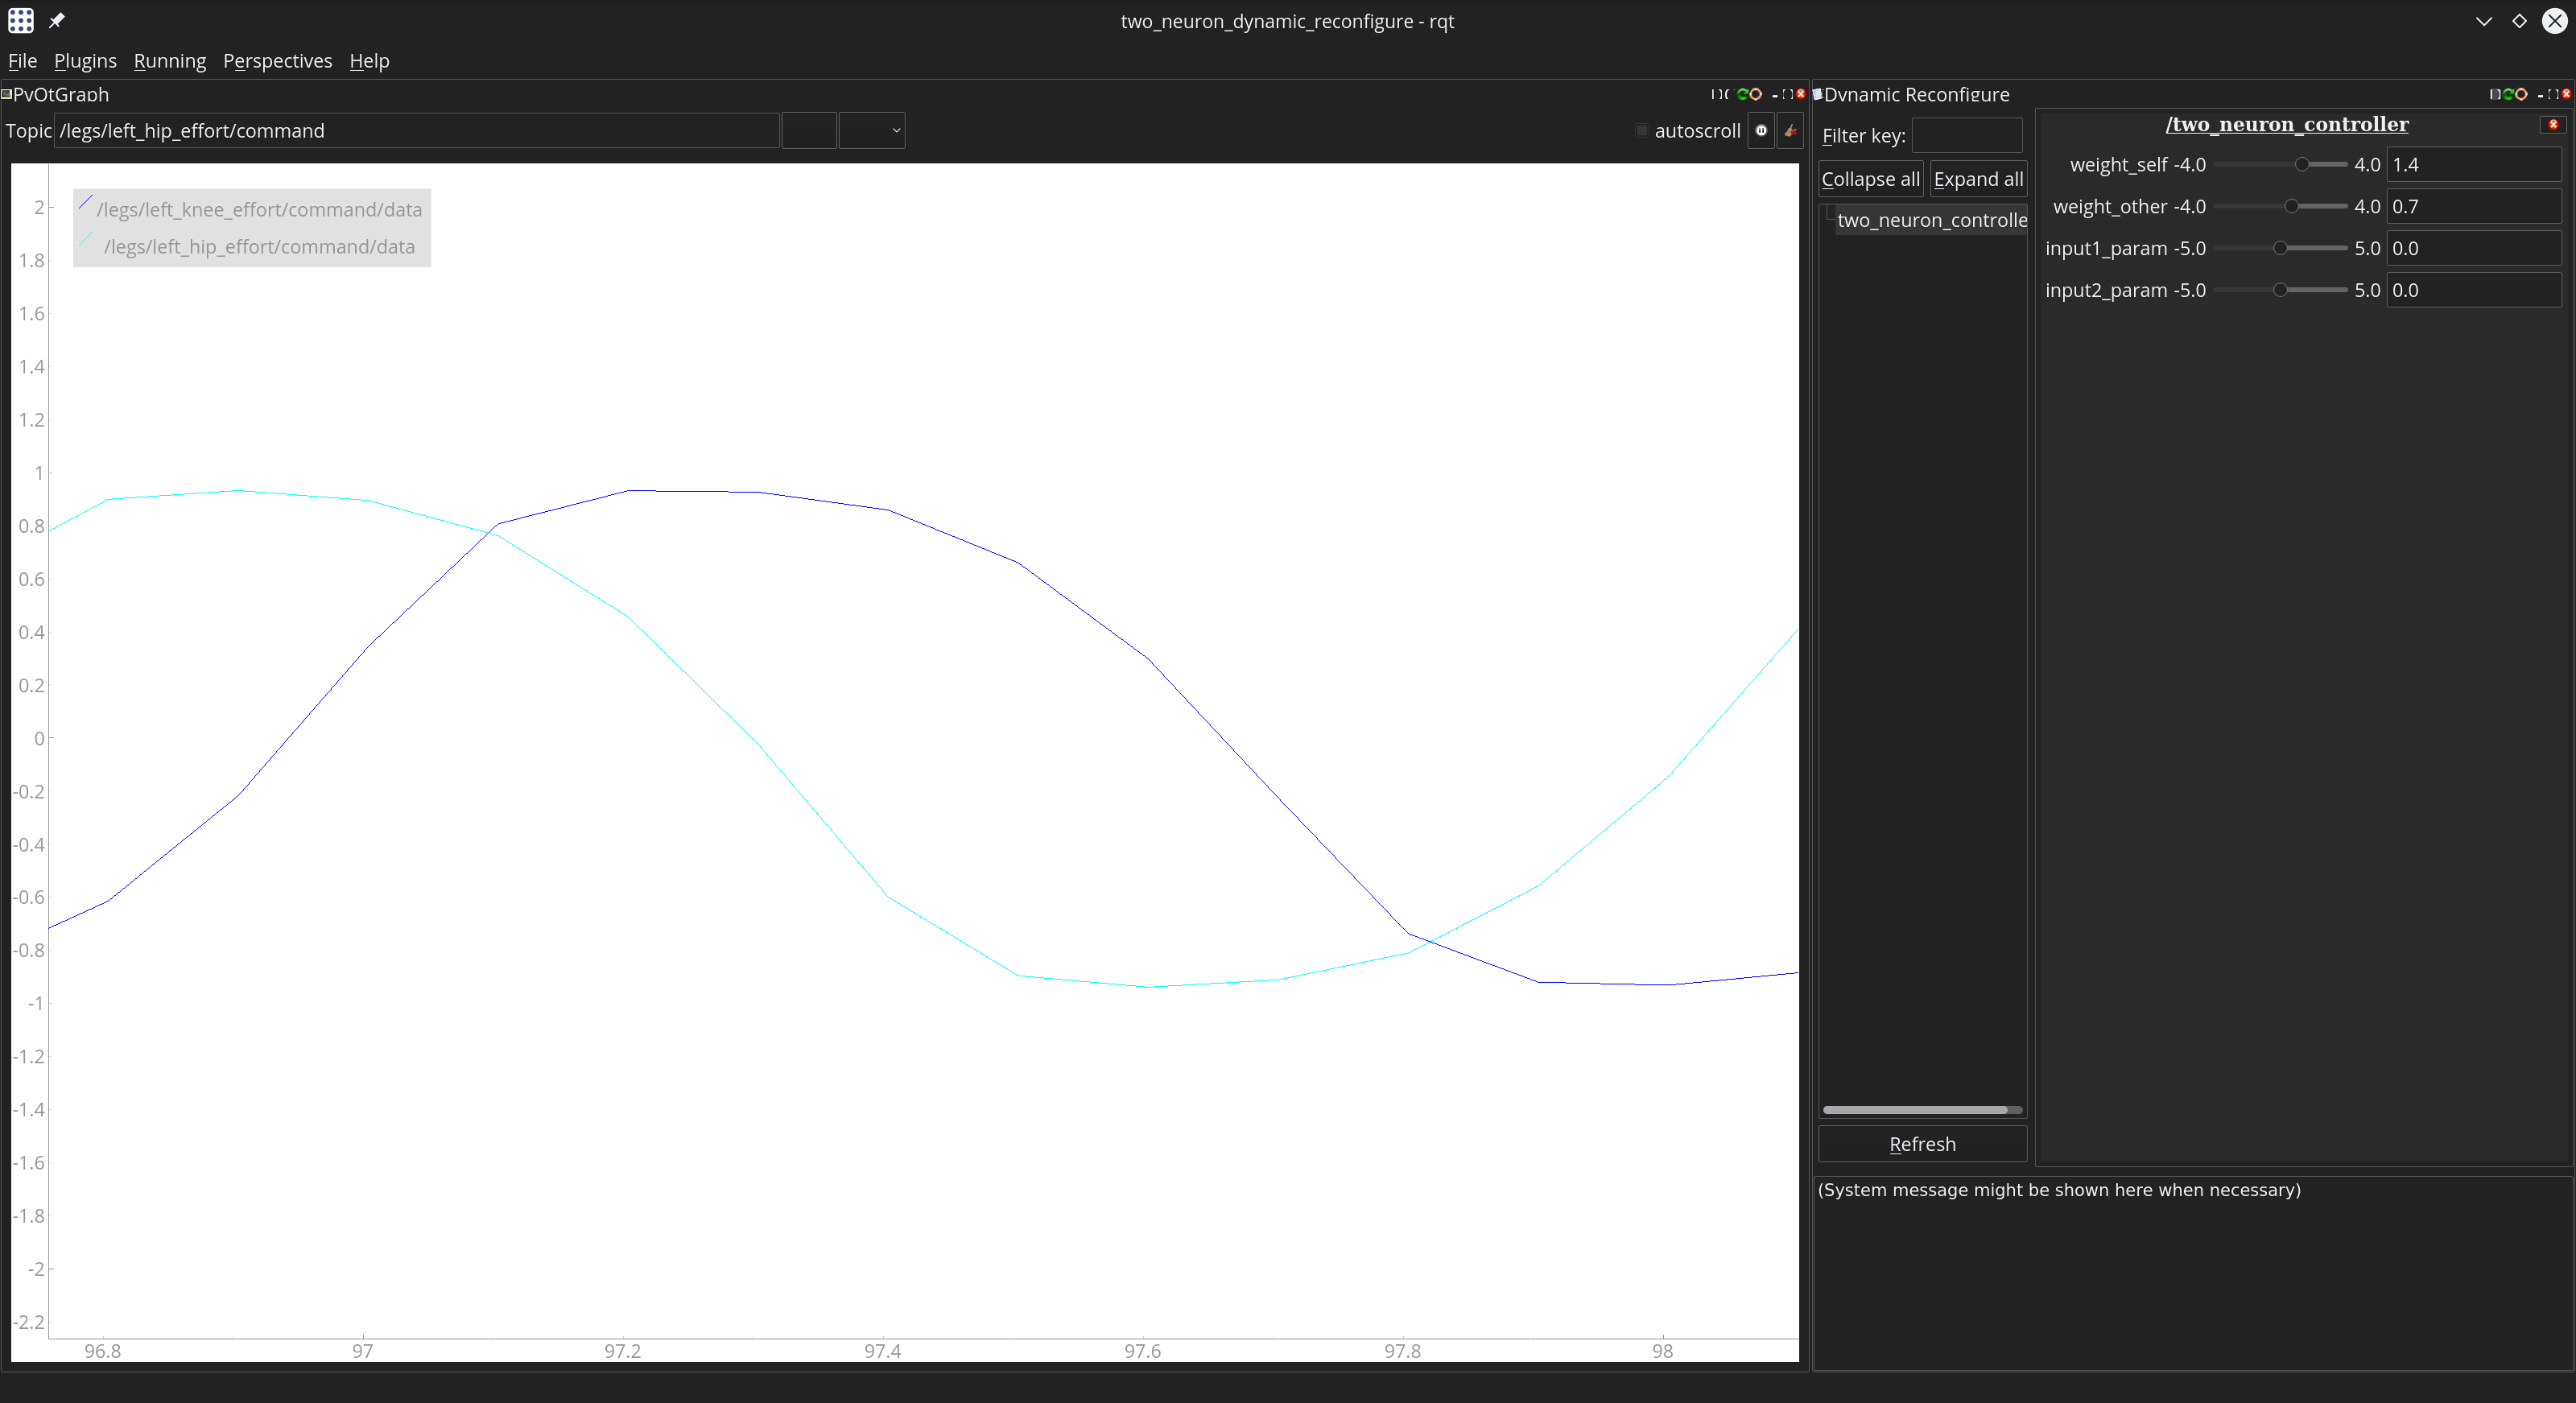
\includegraphics[width=\textwidth]{figures/rqt_interface}
    \caption{RQT workspace containing the CPG signals and the dynamic recofigurable parameters.}
    \label{fig:rqt_interface}
\end{figure}

These are also used to change the behavior of the ANN in order to be adapted to changes in Gazebo.
Gazebo users can modify the relationship between the simulation and computation times.
This is adjusted with a \textit{real time factor} that is read by the node and used to adjust the frequencies of the CPGs.
% subsubsection two_neuron_controller (end)

\subsubsection{Impulse controller} % (fold)
\label{ssub:impulse_controller}
Among other things this node shows how to:
\begin{enumerate}
    \item Load and unload different joint controllers.
    \item Give some wrappings for set of controllers (hoping position).
    \item Offer services for jumping: given a file or given the values and impulse time.
\end{enumerate}
This node implements some methods that enable it to change on-the-fly the handlers of each individual joint.
Furthermore, three combinations of individual joint handlers are given, being these: (1) all in position mode, (2) all in effort mode and (3) left leg in position mode and right in effort mode.
The last one is useful when hopping, a moment in which a leg must hold a position and the other keep pushing in order to jump.

Three different services are implemented in order to simulate peak torques in the joints to generate an impulse on the robot and model jump dynamics.
The first two are \textit{impulse\_one\_leg} and \textit{impulse\_two\_legs} which, given a torque for each joint and an impulse time, give the possibility to jump either with one or two legs.
Both services load the necessary joint controllers in order to achieve the desired movements.
The third one offers the same service but the parameters are read from a file instead.
This is very convenient when combined with the dynamic controllers that can be developed in MatLab and explained in the section \ref{sec_dynamic_controller}.
% subsubsection impulse_controller (end)

% subsection example_controllers (end)